\documentclass{beamer} 
\usepackage{tikz}
\usepackage[all]{xy}
\usepackage{amsmath,amssymb}
\usepackage{hyperref}
\usepackage{graphicx}
\usepackage{algorithmic}
\usepackage{multirow}

\DeclareMathOperator*{\argmin}{arg\,min}
\DeclareMathOperator*{\Lik}{Lik}
\DeclareMathOperator*{\PoissonLoss}{PoissonLoss}
\DeclareMathOperator*{\Peaks}{Peaks}
\DeclareMathOperator*{\Segments}{Segments}
\DeclareMathOperator*{\argmax}{arg\,max}
\DeclareMathOperator*{\maximize}{maximize}
\DeclareMathOperator*{\minimize}{minimize}
\newcommand{\sign}{\operatorname{sign}}
\newcommand{\RR}{\mathbb R}
\newcommand{\ZZ}{\mathbb Z}
\newcommand{\NN}{\mathbb N}
\newcommand{\z}{$z = 2, 4, 3, 5, 1$} 

\newcommand{\algo}[1]{\textcolor{#1}{#1}}
\definecolor{PDPA}{HTML}{66C2A5}
\definecolor{CDPA}{HTML}{FC8D62}
\definecolor{GPDPA}{HTML}{4D4D4D}

% Set transparency of non-highlighted sections in the table of
% contents slide.
\setbeamertemplate{section in toc shaded}[default][100]
\AtBeginSection[]
{
  \setbeamercolor{section in toc}{fg=red} 
  \setbeamercolor{section in toc shaded}{fg=black} 
  \begin{frame}
    \tableofcontents[currentsection]
  \end{frame}
}

\begin{document}

\title{Convolutional neural networks}

\author{
  Toby Dylan Hocking\\
  toby.hocking@nau.edu\\
  toby.hocking@r-project.org\\
}

\maketitle


\begin{frame}
  \frametitle{Supervised learning setup}
  \begin{itemize}
  \item Have an input $\mathbf x\in\mathbb R^d$ -- a vector of $d$
    real numbers.
  \item And an output $y$ (real number: regression, integer ID:
    classification).
  \item Want to learn a prediction function $f(\mathbf x) = y$ that
    will work on a new input.
  \item In a neural network with $L-1$ hidden layers the function $f$
    is defined using composition of $L$ functions,
    $f(x)=f^{(L)}[\cdots f^{(1)}[x] ]\in\mathbb R$.
  \end{itemize}
\end{frame}

\begin{frame}
  \frametitle{Each function is matrix multiplication and activation}
  \begin{itemize}
  \item Prediction function $f(x)=f^{(L)}[\cdots f^{(1)}[x] ]\in\mathbb R$.
  \item Each function $l\in\{1,\dots, L\}$ is a matrix multiplication
    followed by an activation function:
    $f^{(l)}[z] = \sigma^{(l)}[ W^{(l)} z ]$ where
    $W^{(l)}\in\mathbb R^{u^{(l)}\times u^{(l-1)}}$ is a weight matrix
    to learn, and $z\in\mathbb R^{u^{(l-1)}}$ is the input vector to
    that layer.
  \item So far we have only discussed fully connected networks, which
    means that each entry of the weight matrix is unique and non-zero.
  \item This week we discuss ``convolutional'' networks which are
    useful for spatial data and can be interpreted as multiplication
    by a special kind of matrix (with sparsity and weight sharing).
\end{itemize}
\end{frame}

\begin{frame}
  \frametitle{Convolution is a linear operator for spatial data}
  Useful for data which have spatial dimension(s) such as time series
  (1 dim) or images (2 dim). Simple example with 1 dim:
  \begin{itemize}
  \item $\mathbf x = [ x_1, \dots, x_D ]$ is an input vector (array of $D$ data).
  \item $\mathbf v = [ v_1, \dots, v_P ]$ is a kernel (array of $P$ parameters
    / weights to learn), $P<D$.
  \item $\mathbf h = [ h_1, \dots, h_U ]$ is an output vector of $U=D-P+1$ 
    hidden units. Convolution (actually cross-correlation) is used to
    define each hidden unit:
    $\forall u\in\{1,\dots,U\}, h_u = \sum_{p=1}^P v_p x_{u+p-1} $.
\item EX: $D=3$ inputs, $P=2$ parameters $\Rightarrow U=2$ output units:
  \begin{eqnarray*}
    h_1 &=& v_1 x_1 + v_2 x_2 \text{ (convolutional=sparse+shared)}\\ 
    h_2 &=& v_1 x_2 + v_2 x_3 \text{ (convolutional=sparse+shared)}\\
    h_1 &=& w_{1,1} x_1 + w_{1,2} x_2 + w_{1,3} x_3 \text{ (fully connected/dense)}\\ 
    h_2 &=& w_{2,1} x_1 + w_{2,2} x_2 + w_{2,3} x_3 \text{ (fully connected/dense)} 
  \end{eqnarray*}
\item Compare with fully connected -- convolutional means weights are
  shared among outputs, and some are zero/sparse.
  \end{itemize}
\end{frame}

\begin{frame}
  \frametitle{Difference in connectivity and weight sharing}
  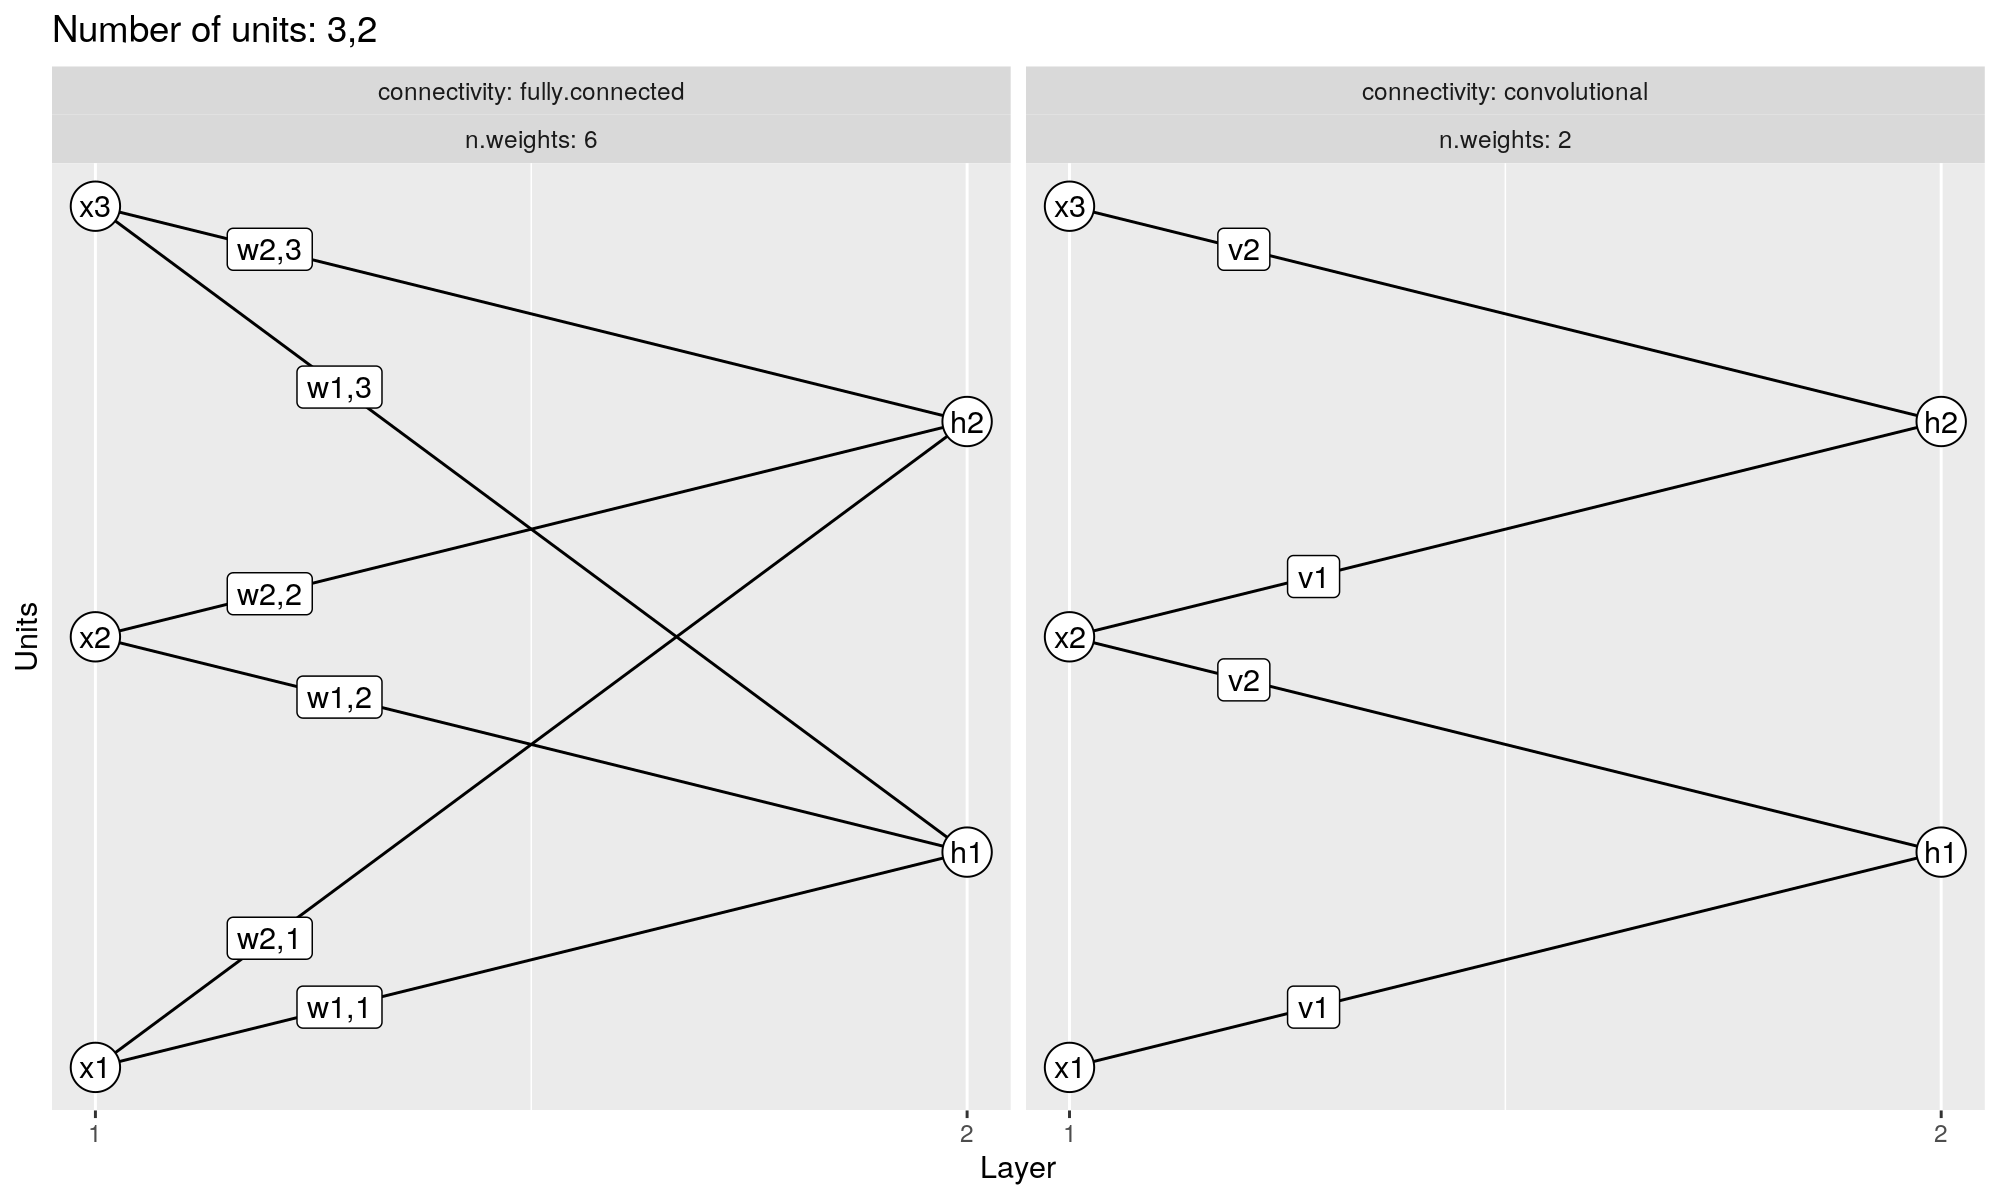
\includegraphics[width=\textwidth]{figure-convolutional-3-2}
\end{frame}

\begin{frame}[fragile]
  \frametitle{Matrix interpretation of convolution}
  \begin{eqnarray*}
  \begin{bmatrix}
    h_1 \\
    h_2 
  \end{bmatrix}
    &=&
  \begin{bmatrix}
    w_{1,1} & w_{1,2} & w_{1,3} \\
    w_{2,1} & w_{2,2} & w_{2,3}
  \end{bmatrix}
  \begin{bmatrix}
    x_1 \\
    x_2 \\
    x_3
  \end{bmatrix} \text{(fully connected)}
    \\
  \begin{bmatrix}
    h_1 \\
    h_2 
  \end{bmatrix}
    &=&
  \begin{bmatrix}
    v_{1} & v_{2} & 0 \\
    0 & v_{1} & v_{2}
  \end{bmatrix}
  \begin{bmatrix}
    x_1 \\
    x_2 \\
    x_3
  \end{bmatrix} \text{(convolutional)}
  \end{eqnarray*}
  \begin{itemize}
  \item Weight sharing: same weights used to compute different
    output units.
  \item Sparsity: zeros in weight matrix.
  \end{itemize}

\begin{verbatim}
torch.nn.Conv1d(
  in_channels=1, 
  out_channels=1,
  kernel_size=2)
\end{verbatim}
  
\end{frame}

\begin{frame}
  \frametitle{Multiple kernels/filters or sets of weights}
  \begin{itemize}
  \item $x = [ x_1, \dots, x_D ]$ is an input vector (array of $D$ data).
  \item $v = \begin{bmatrix}
      v_{1,1} & \cdots & v_{1,P} \\
      \vdots & \ddots & \vdots \\
      v_{K,1} & \cdots & v_{K,P}
    \end{bmatrix}$ is a matrix of $K$ kernels,\\each row is an array of
    $P$ parameters / weights to learn, $P<D$.
  \item $h = \begin{bmatrix}
      h_{1,1} & \dots & h_{1,U} \\
      \vdots & \ddots & \vdots \\
      h_{K,1} & \cdots & h_{K,U}
      \end{bmatrix}$ is an output matrix of
      hidden units. \\
      Each row is computing by applying a kernel to the input:
      $$
      \forall u\in\{1,\dots,U\},
      \forall k\in\{1,\dots,K\},
      h_{k,u} = \sum_{p=1}^P v_{k,p} x_{u+p-1}
      $$
    \item EX in previous slide: $D=3$ inputs, $P=2$ parameters per
      kernel, $K=2$ kernels $\Rightarrow U=2$ output units per kernel,
      4 output units total.
  \end{itemize}
\end{frame}

\begin{frame}[fragile]
  \frametitle{Colors for unique weight parameters to learn}
  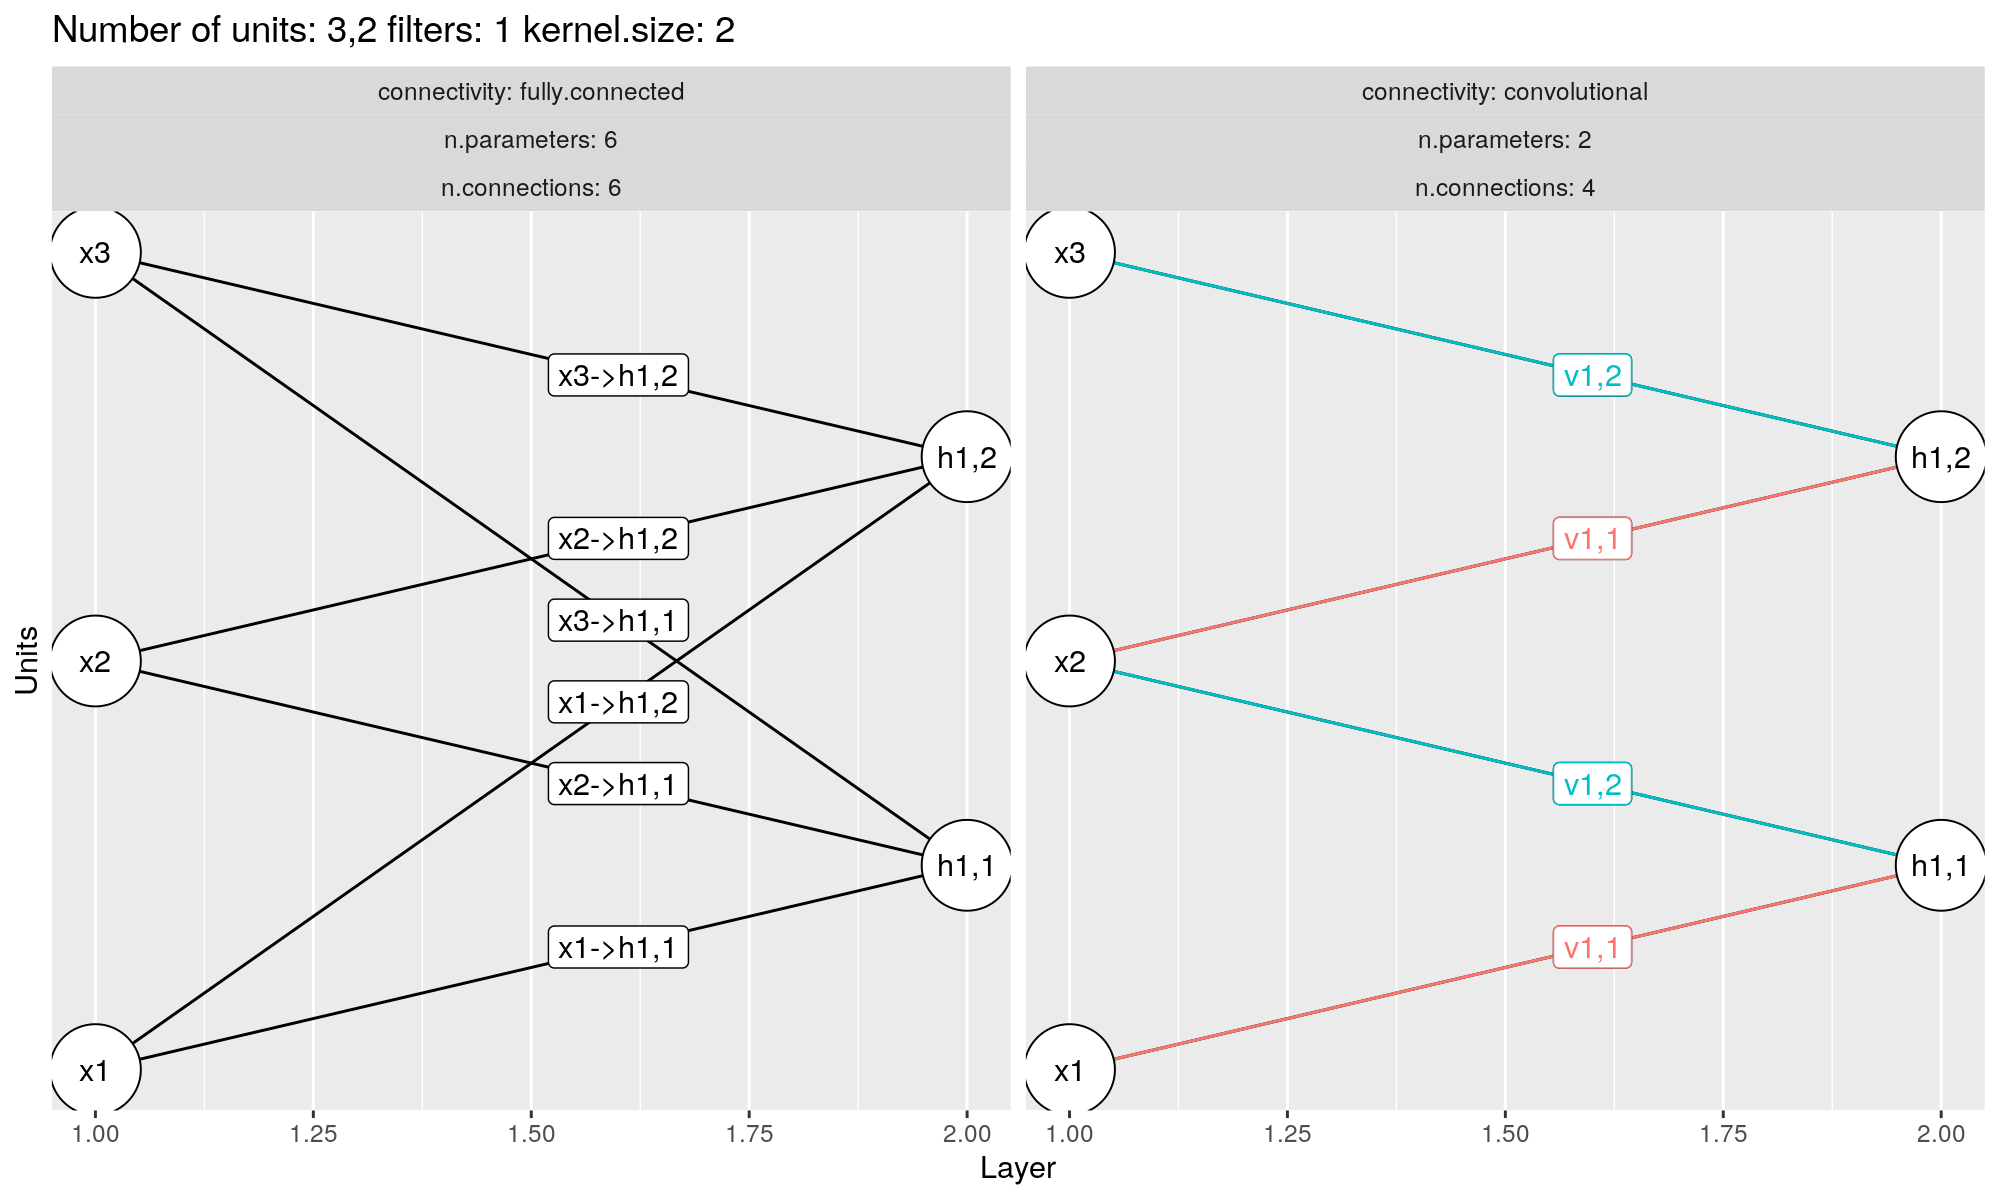
\includegraphics[width=\textwidth]{figure-convolutional-filters-3-2-1}
\begin{verbatim}
torch.nn.Conv1d(in_channels=1, 
  out_channels=1, kernel_size=2)
\end{verbatim}

\end{frame}

\begin{frame}[fragile]
  \frametitle{Colors for unique weight parameters to learn}
  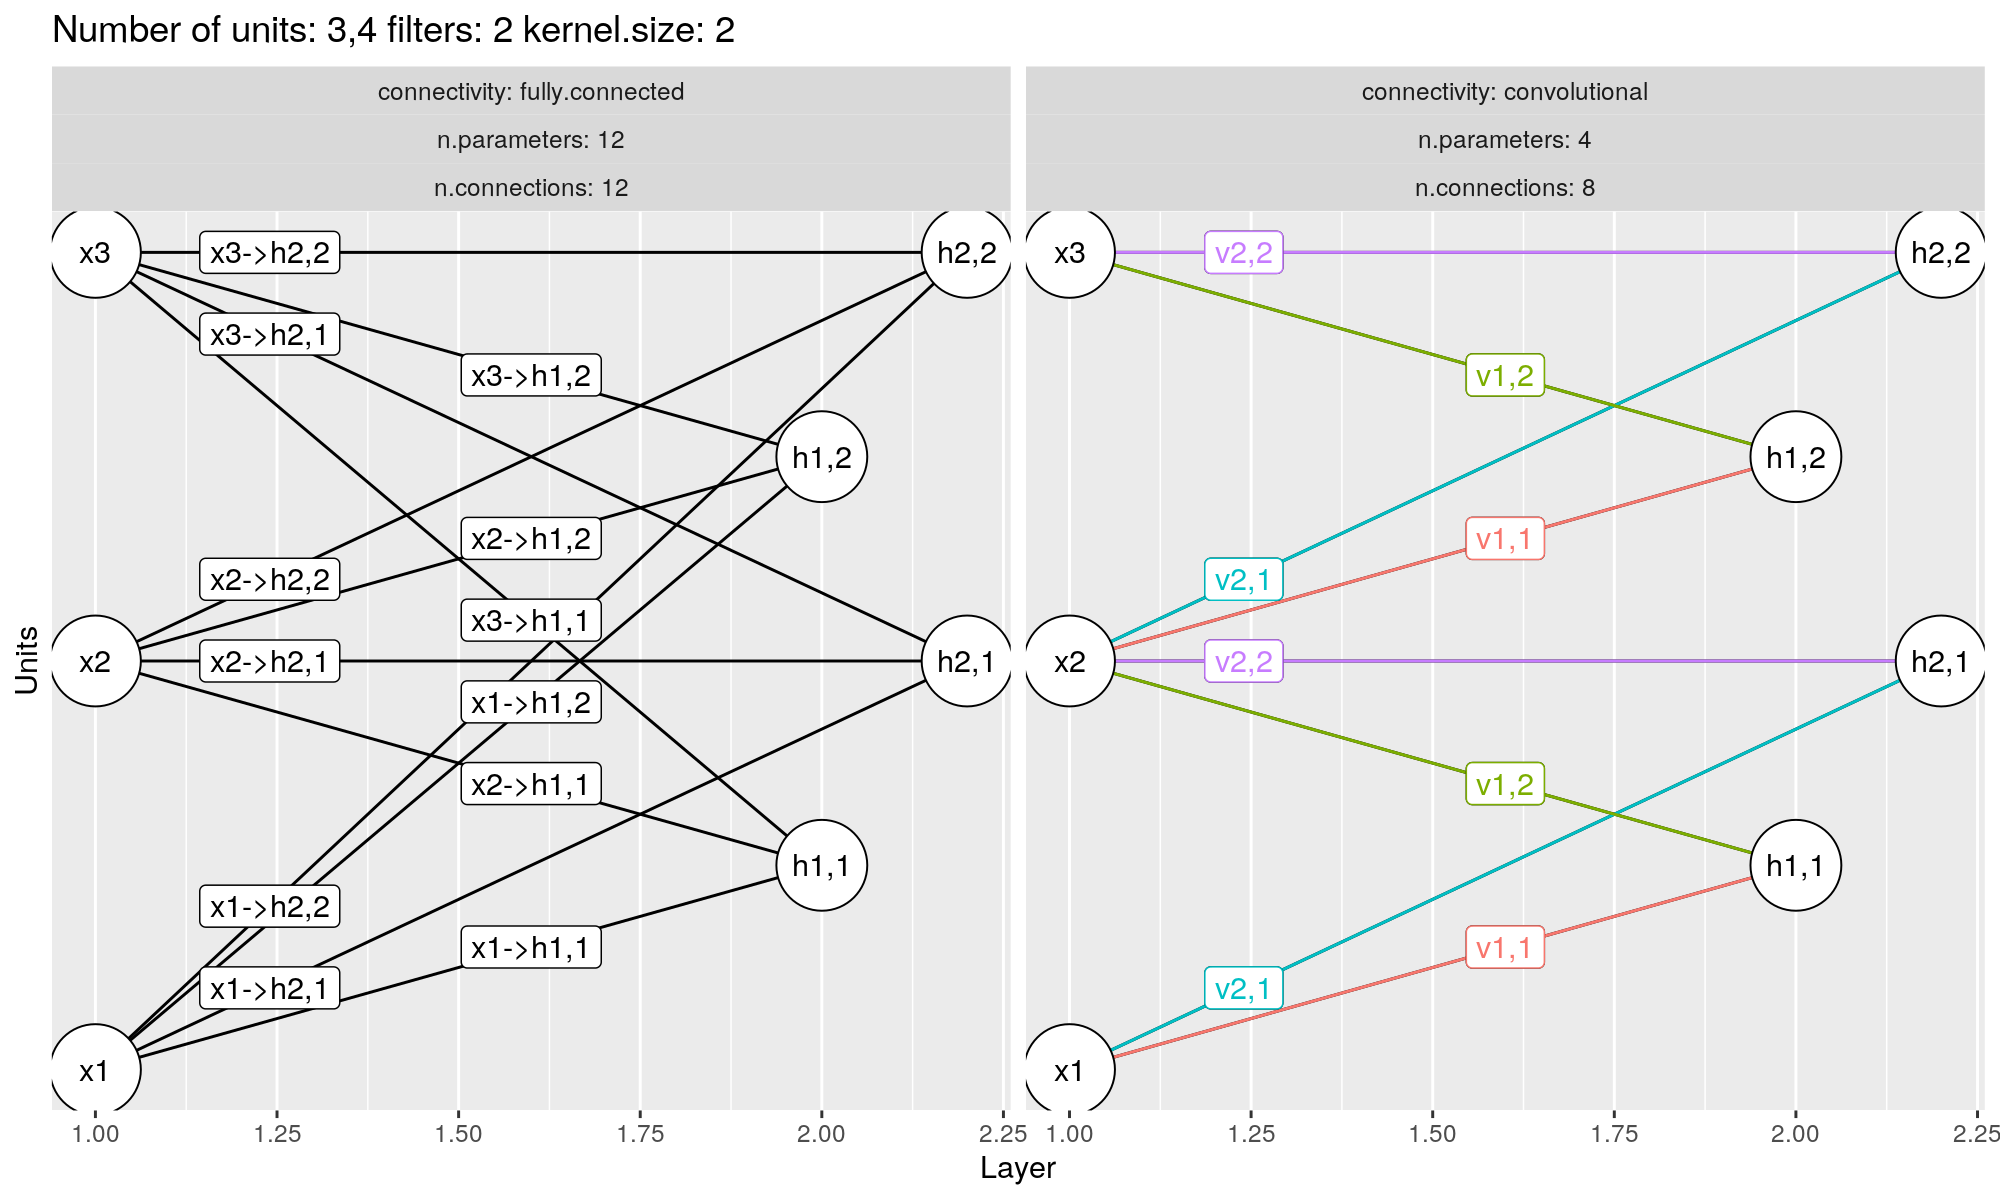
\includegraphics[width=\textwidth]{figure-convolutional-filters-3-2-2}
  
\begin{verbatim}
torch.nn.Conv1d(in_channels=1, 
  out_channels=2, kernel_size=2)
\end{verbatim}
\end{frame}

\begin{frame}[fragile]
  \frametitle{Matrix interpretation of convolution}
  \begin{eqnarray*}
  \begin{bmatrix}
    h_{1,1} \\
    h_{1,2} \\
    h_{2,1} \\
    h_{2,2}
  \end{bmatrix}
    &=&
  \begin{bmatrix}
    v_{1,1} & v_{1,2} & 0 \\
    0 & v_{1,1} & v_{1,2} \\
    v_{2,1} & v_{2,2} & 0 \\
    0 & v_{2,1} & v_{2,2}
  \end{bmatrix}
  \begin{bmatrix}
    x_1 \\
    x_2 \\
    x_3
  \end{bmatrix} \text{(convolutional)}
  \end{eqnarray*}
  \begin{itemize}
  \item Weight sharing: same weights used to compute different
    output units. 
  \item Sparsity: zeros in weight matrix.
  \end{itemize}

\begin{verbatim}
torch.nn.Conv1d(
  in_channels=1, 
  out_channels=2,
  kernel_size=2)
\end{verbatim}
  
\end{frame}

\begin{frame}
  \frametitle{Video about convolution}
  \url{https://github.com/tdhock/useR2017-debrief}

  Angus Taylor's talk at useR 2017.

  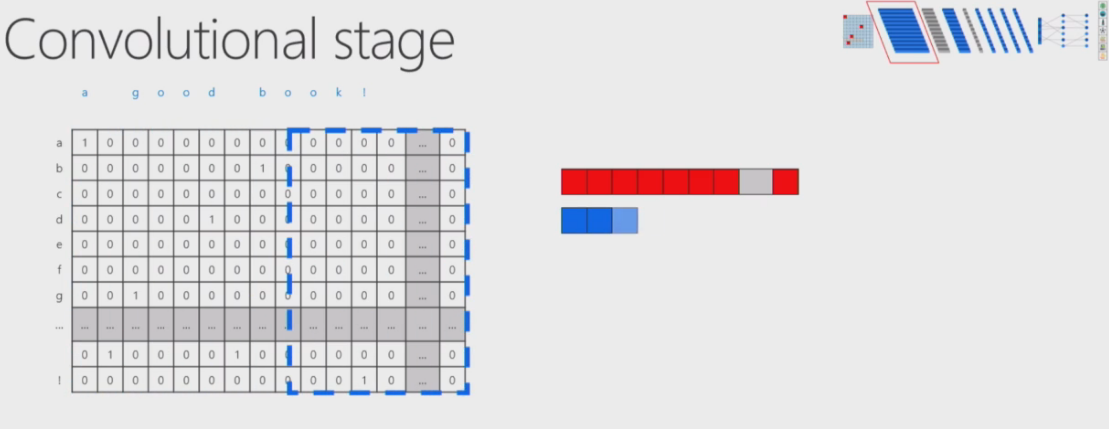
\includegraphics[width=\textwidth]{screenshot-conv} 
\end{frame}

\begin{frame}[fragile,fragile]
  \frametitle{A more complex example (one filter)}
  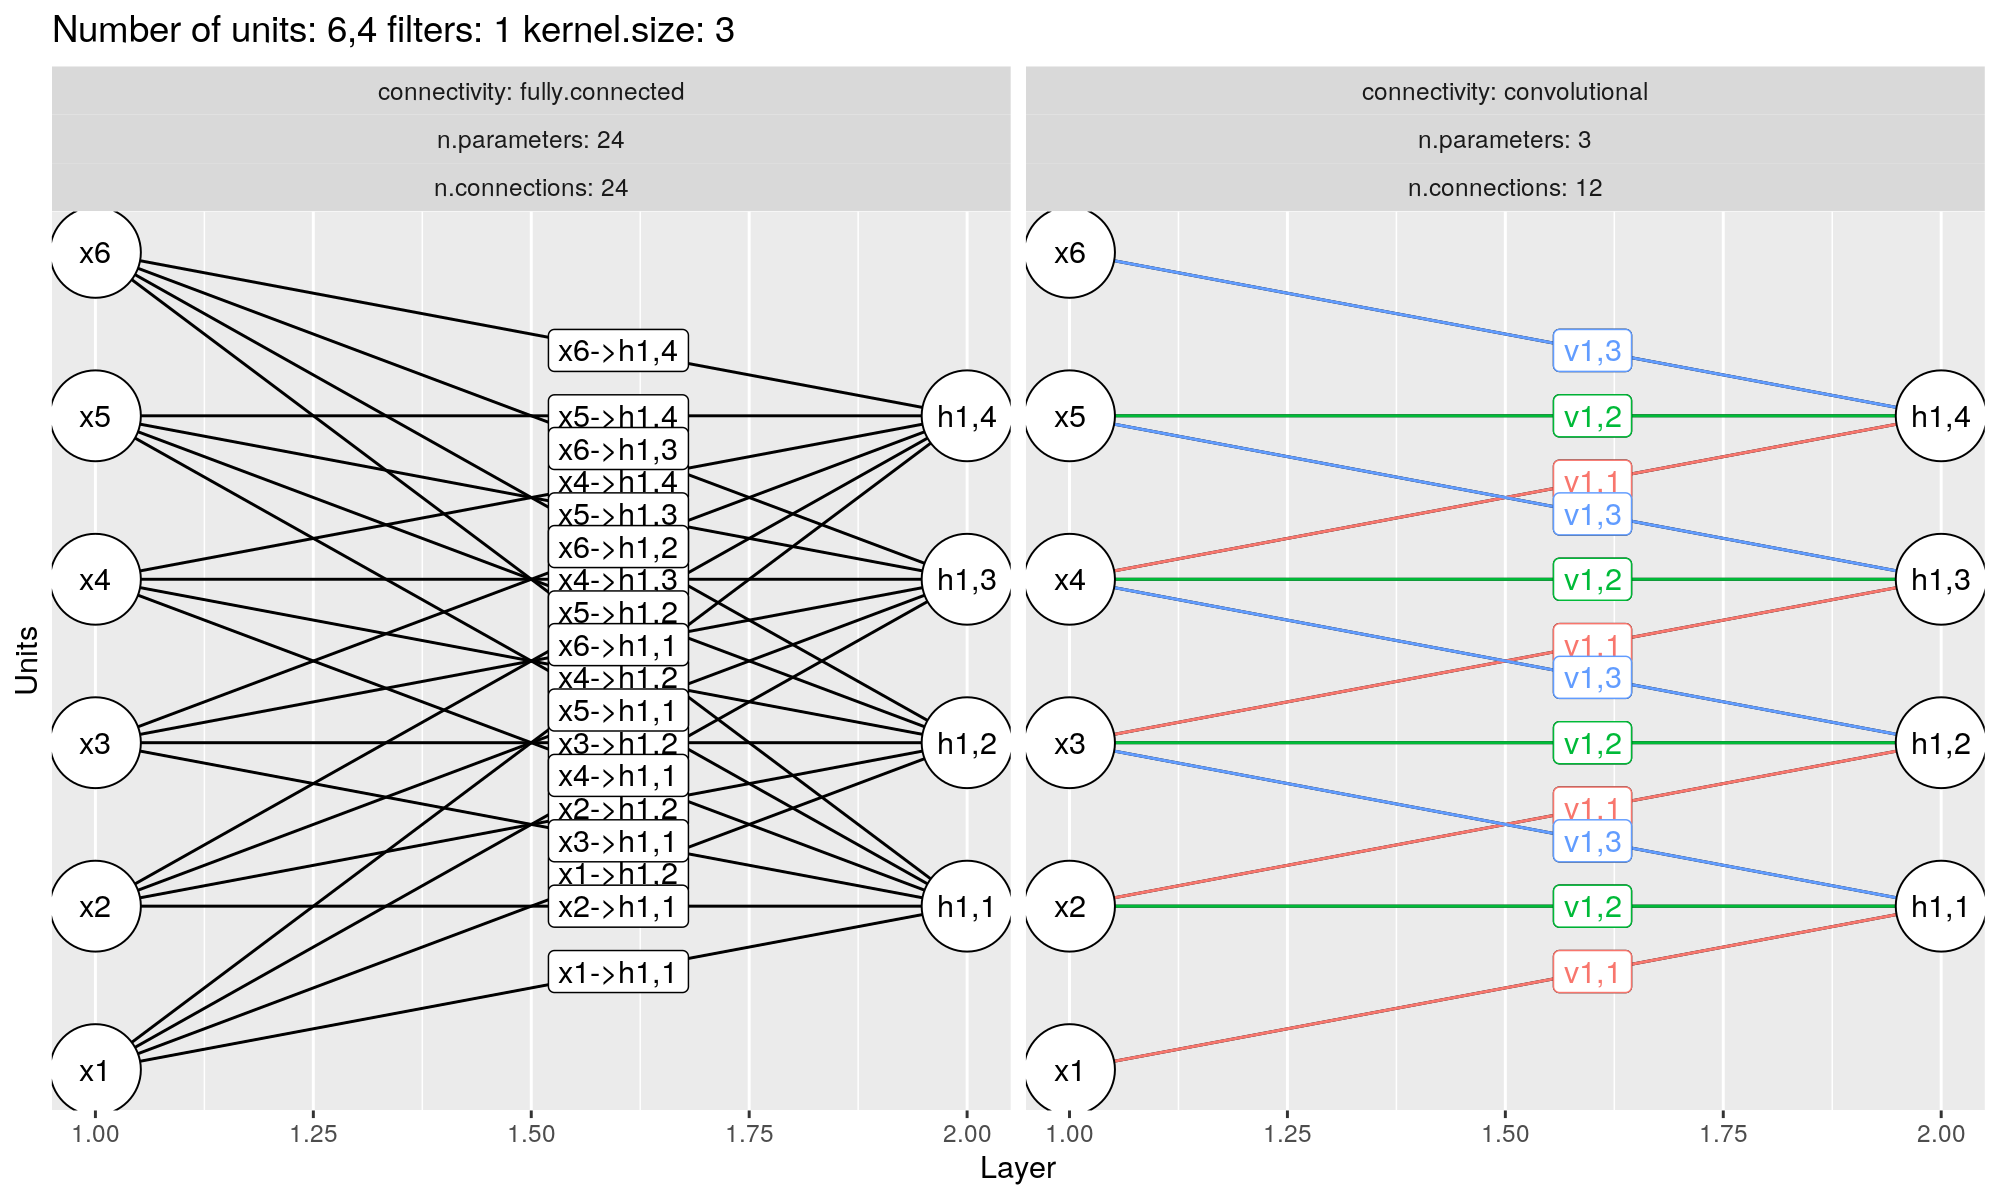
\includegraphics[width=\textwidth]{figure-convolutional-filters-6-3-1}

\begin{verbatim}
torch.nn.Conv1d(in_channels=1, 
  out_channels=1, kernel_size=3)
\end{verbatim}
  
\end{frame}

\begin{frame}[fragile]
  \frametitle{A more complex example (two filters)}
  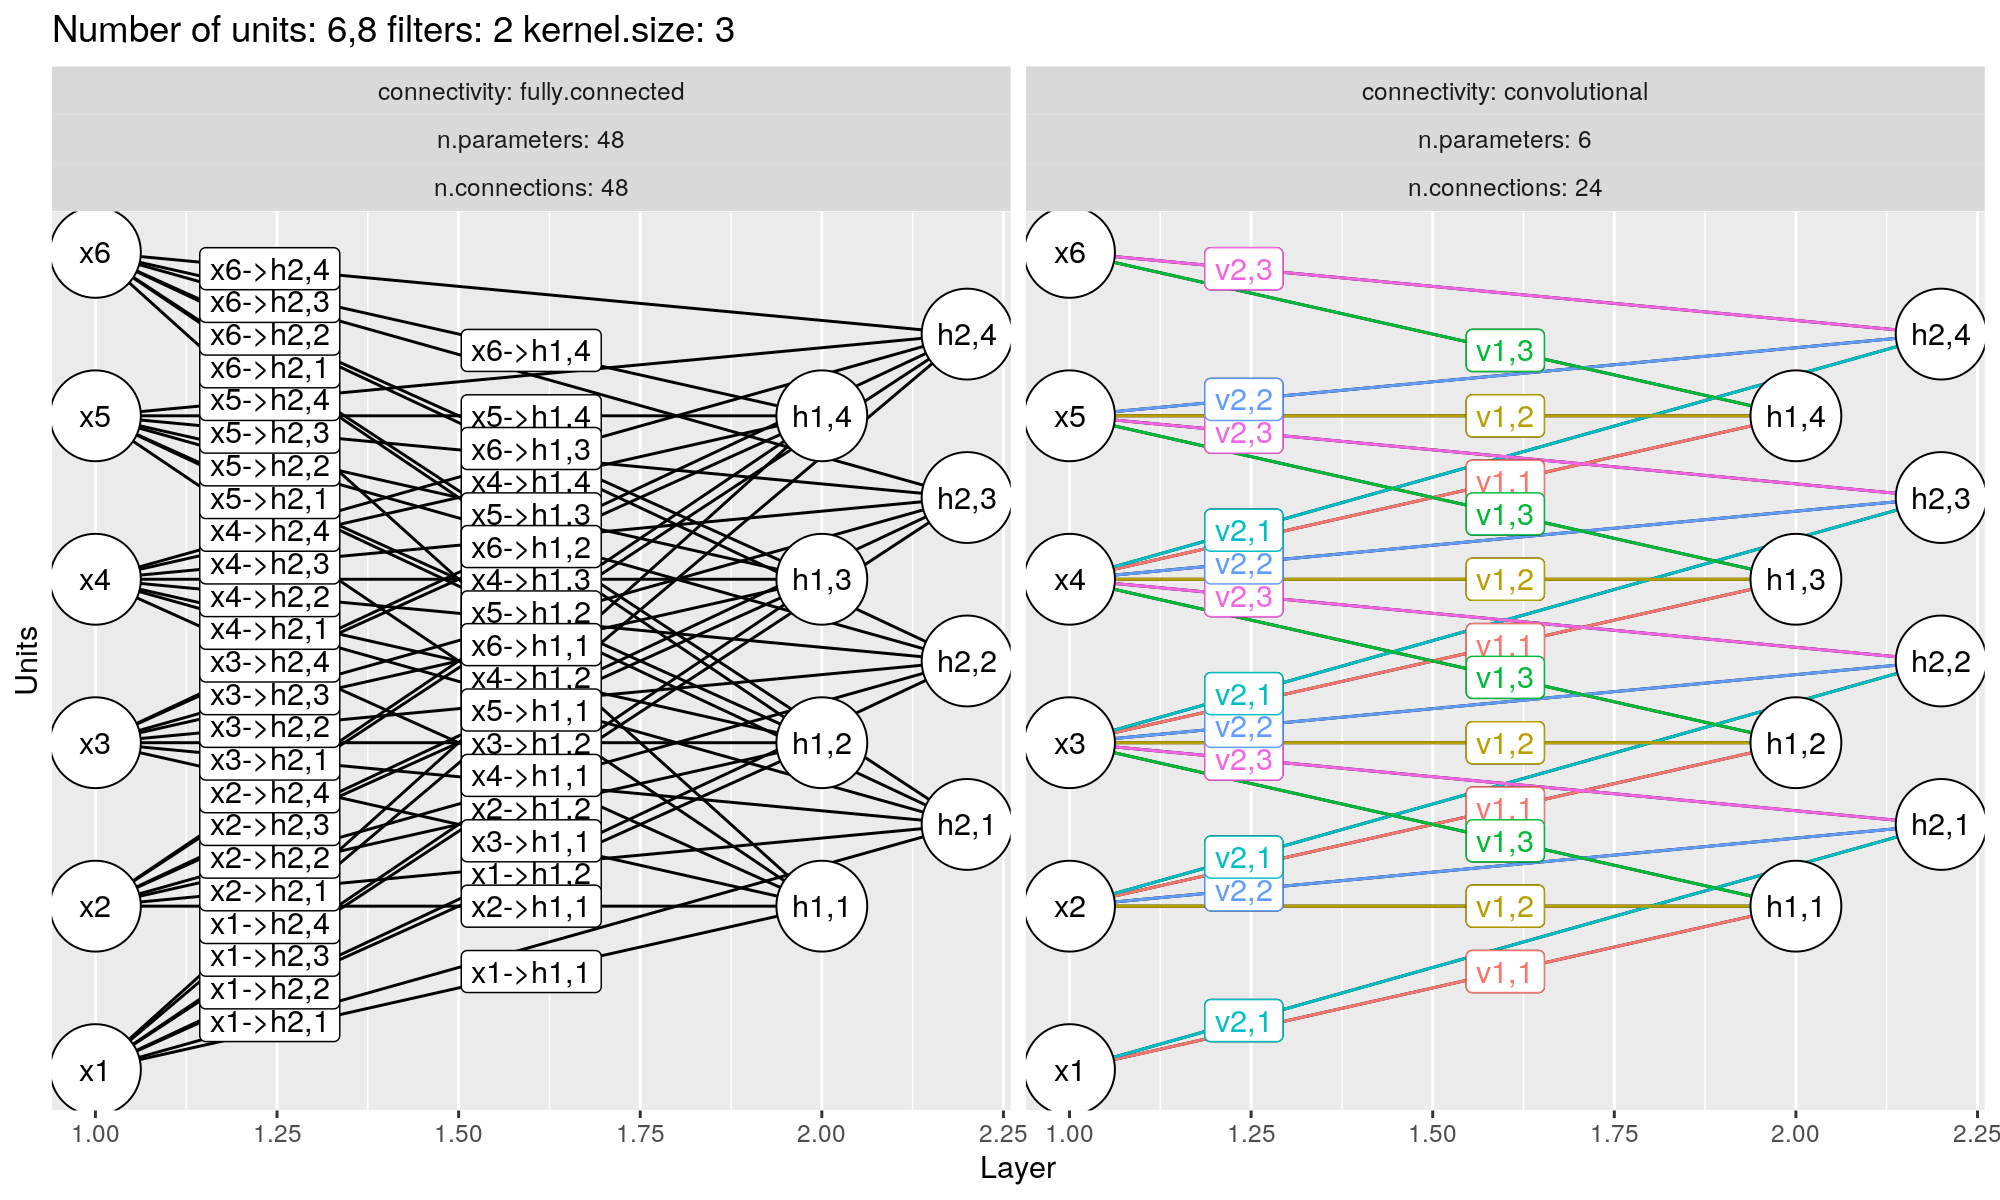
\includegraphics[width=\textwidth]{figure-convolutional-filters-6-3-2}
   
\begin{verbatim}
torch.nn.Conv1d(in_channels=1, 
  out_channels=2, kernel_size=3)
\end{verbatim}
  
\end{frame}

\begin{frame}
  \frametitle{Architecture exercises}
  1D Convolution: if there are $D=10$ inputs and $U=5$ outputs, 
  \begin{itemize}
  \item how many parameters to learn in a fully
    connected layer?
  \item a single kernel in a convolutional layer,
    \begin{enumerate}
    \item how many parameters are there to learn?
    \item how many connections in the network diagram
      representation?
    \item how many zeros in the weight matrix
      representation?
    \end{enumerate}
  \end{itemize}

  2D Convolution: if you have a 10 x 10 pixel input image, and you
  apply 5 x 5 kernel,
  \begin{enumerate}
  \item How many parameters are there to learn in each filter?
  \item How many parameters total if there are 20 filters?
  \item How many output units per filter?
  \item How many output units total using 20 filters?
  \end{enumerate}
\end{frame}

\begin{frame}
  \frametitle{Computation exercises (forward propagation)}
  \begin{eqnarray*}
    \mathbf x &=& \begin{bmatrix}
      0 \\
      3 \\
      10
    \end{bmatrix}\\
    \mathbf w &=& \begin{bmatrix}
      -1 & 2 & -3 \\
      4 & -5 & 6
    \end{bmatrix}\\
    \mathbf v &=& \begin{bmatrix}
      -2 \\
      1
    \end{bmatrix}\\
  \end{eqnarray*}
  If $\mathbf x$ is an input vector,
  \begin{enumerate}
  \item what is the output vector when using $\mathbf w$ as the weight
    matrix in a fully connected layer?
  \item what is the output vector when using $\mathbf v$ as the kernel
    in a 1d convolutional layer?
  \end{enumerate}
\end{frame}
  
\begin{frame}
  \frametitle{Pooling}
  Typical order of application in a layer is
  \begin{enumerate}
  \item Weight matrix multiplication (learned via gradient descent).
  \item Activation, nonlinear function (not learned).
  \item Pooling, reducing the number of units (not learned).
  \end{enumerate}
  What is pooling? 
  \begin{itemize}
  \item Main purpose: reducing time/space during learning/prediction.
  \item Like convolution in that you apply some operation in a window
    over inputs; each window creates a single output unit.
  \item In convolution the operation is \textbf{multiplication} of inputs in
    window and corresponding weights, then \textbf{addition} to combine results
    in window.
  \item In pooling the operation is \textbf{mean or max} over all inputs in
    window.
  \item Pooling typically used over spatial dimension (independently
    for each channel/filter). 
  \end{itemize}
\end{frame}

\begin{frame}[fragile]
  \frametitle{Stride}
  \begin{itemize}
  \item This is the offset between windows on which the
    convolution/pooling is computed.
  \item Another technique for reducing number of output units and
    therefore time/space required during learning/prediction.
  \item In previous slides we were using stride of 1 (adjacent windows
    overlap each other and have redundant information).
  \item Often stride is set to kernel size (no overlapping windows)
    --- this is the default in torch.
  \end{itemize} 
\begin{verbatim}
torch.nn.MaxPool1d(kernel_size=2, stride=2)
\end{verbatim}
\end{frame}

\begin{frame}[fragile]
  \frametitle{Stride diagram}
  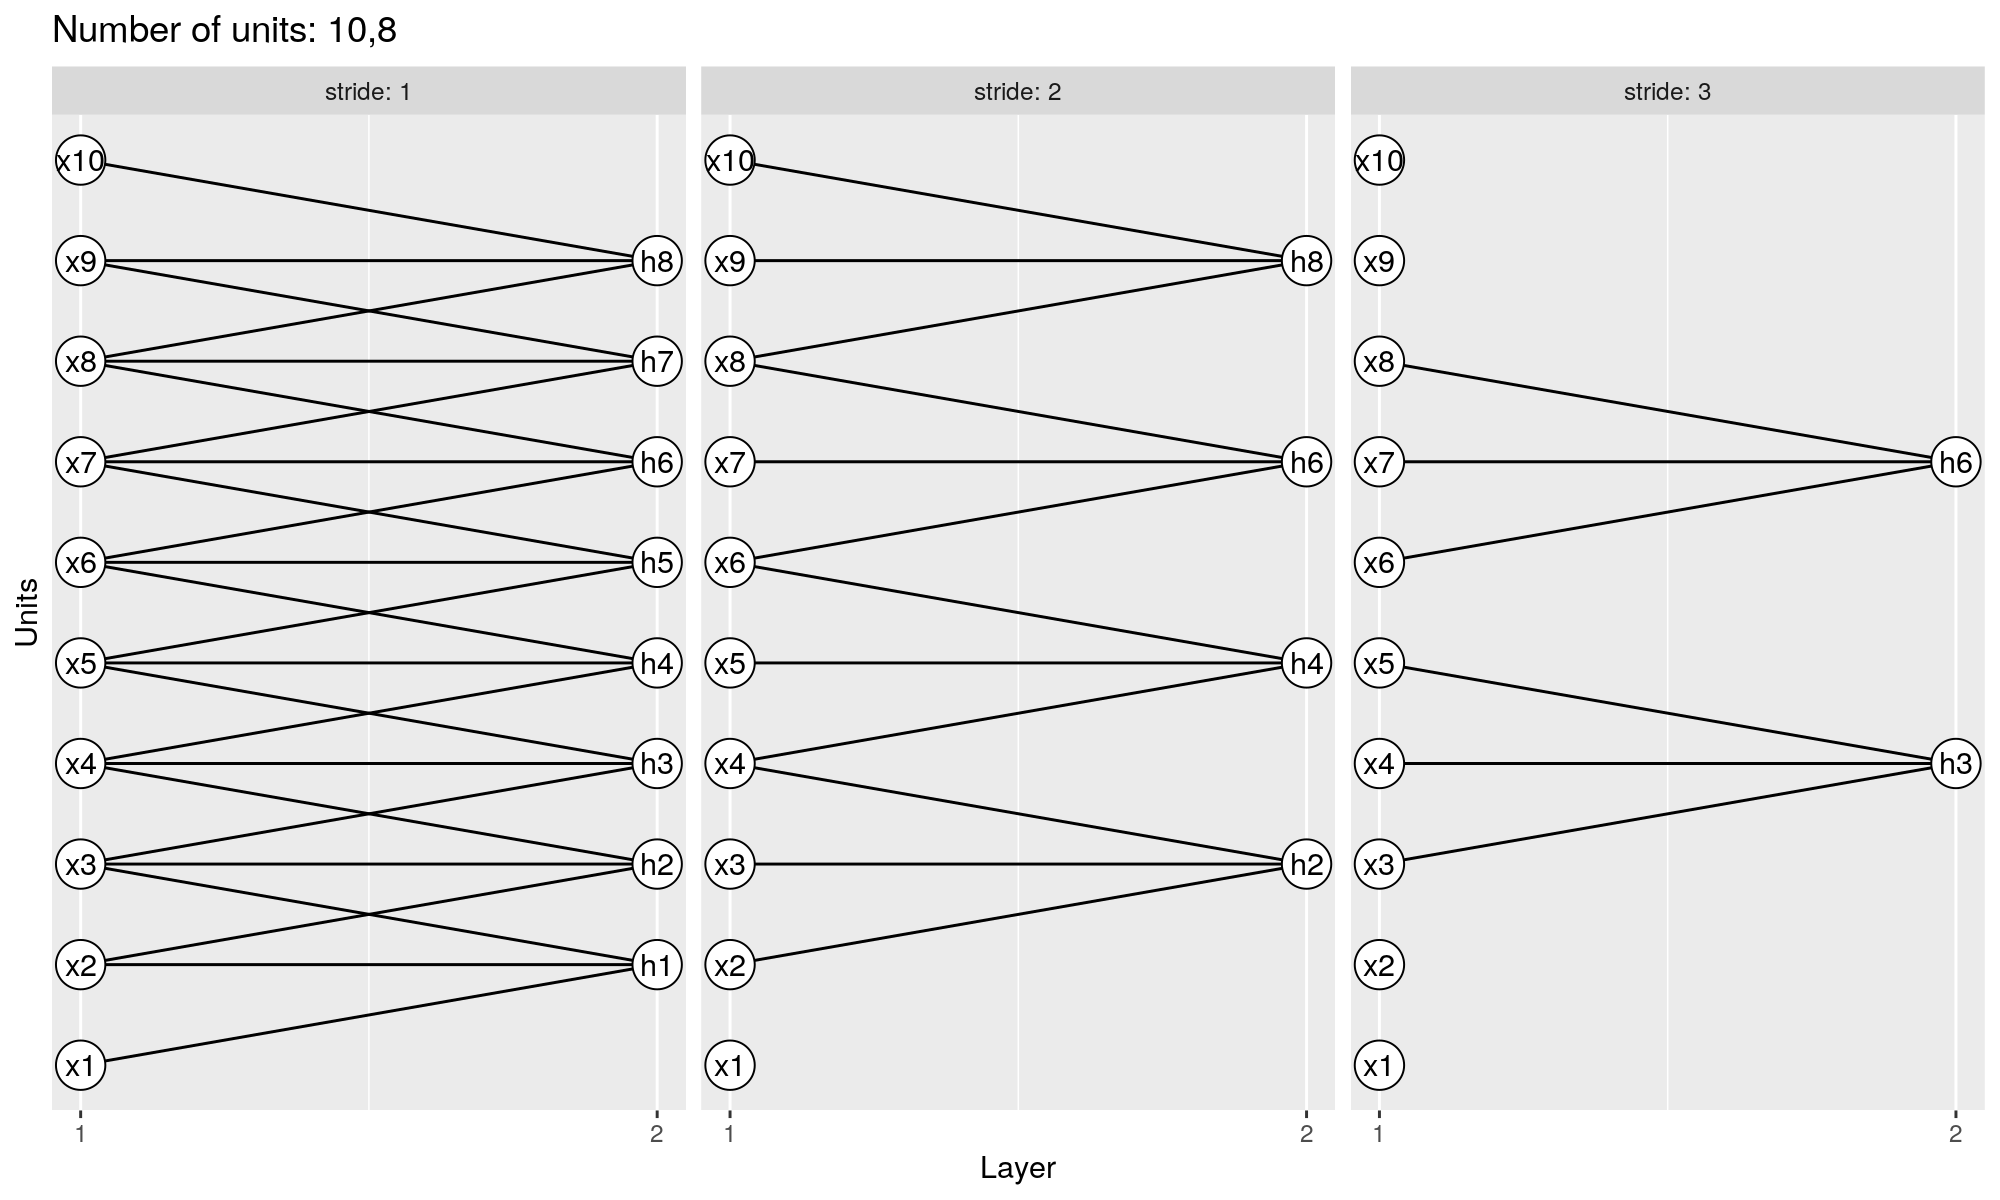
\includegraphics[width=\textwidth]{figure-pooling-10-3}
\begin{verbatim}
torch.nn.MaxPool1d(kernel_size=3, stride=1)
torch.nn.MaxPool1d(kernel_size=3, stride=2)
torch.nn.MaxPool1d(kernel_size=3, stride=3)
\end{verbatim}
\end{frame}

\begin{frame}
  \frametitle{Architecture exercises}
  1D Convolution: if there are $D=20$ inputs and you have a kernel of
  size 5 with stride 5,
  \begin{enumerate}
  \item how many parameters are there to learn?
  \item how many output units are there?
  \item how many connections in the network diagram
    representation?
  \item how many zeros in the weight matrix
    representation?
  \end{enumerate}
  2D Pooling: if you have a 10 x 10 pixel input image, and you apply a
  5 x 5 max pooling kernel with stride 5, how many output units are
  there?
\end{frame}

\begin{frame}
  \frametitle{Computation exercises}
  If $\mathbf x = [0, 3, 10, -2, 5, 1]$ is an input vector,\\
  and $\mathbf k = [-2, 1]$ is a kernel,\\
  \begin{enumerate}
  \item what is the output vector when doing mean pooling with a
    stride of 2 and kernel of size 2?
  \item what is the output vector when doing max pooling with a stride
    of 3 and kernel of size 3?
  \item what is the output vector when using $\mathbf k$ as the kernel
    in a 1d convolutional layer with a stride of 2?
  \end{enumerate}
\end{frame}


\end{document}